\section{Interface Prototypes}

\subsection{Homepage}

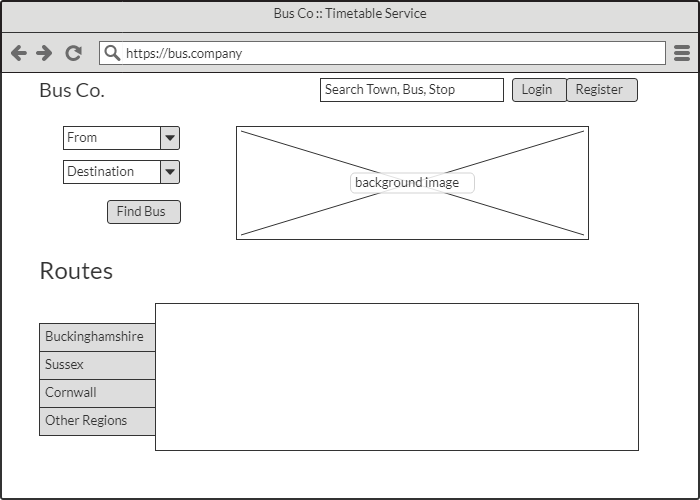
\includegraphics[width=\linewidth]{MockupHomepage.png}

\medskip

The homepage is where customers will be able to find routes from a
specific town or bus stop to another location. In the header, users
can also directly search a route or line to go straight to its route
details page.

\medskip

Below this is a table that lists all the active lines operated by
the bus company. It's broken down by region to allow users to find
their desired routes quickly.

\medskip

For users that are signed in and have added routes to their
favourites, these routes will appear at the top of the route table
in the relevant region.

\subsection{Login}

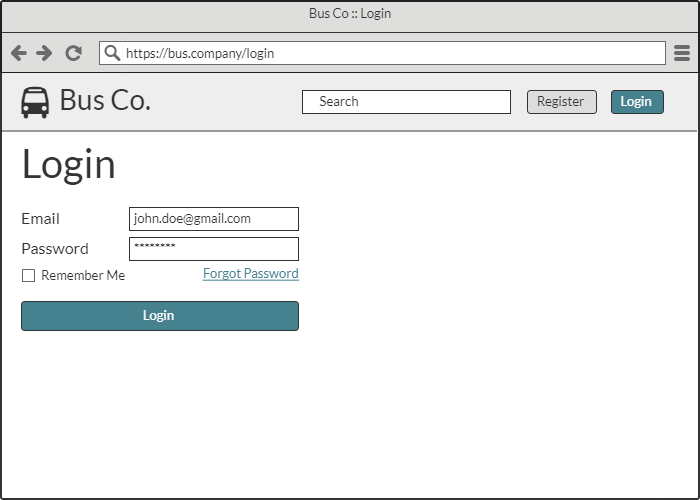
\includegraphics[width=\linewidth]{MockupLogin.png}

\medskip

Staff and users that have previously registered on the service can log in here
with their email and password.

\medskip

Additionally, cookies or localstorage
will be used to remember their login session on repeat visits if
they tick the $Remember Me$ checkbox. Clicking $Forgot Password$
will send an email, which will allow the user to enter a new
password.

\subsection{Register}

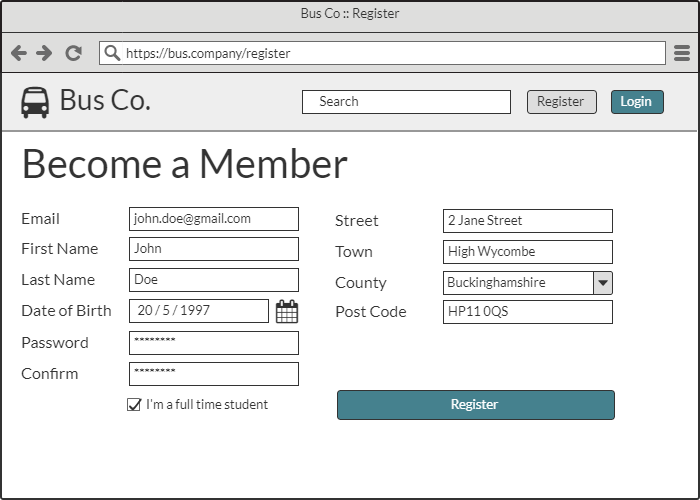
\includegraphics[width=\linewidth]{MockupRegister.png}

\medskip

Registering will add a new user in the database. When registering,
users can enter their details and address. Entering an address will
allow the region they reside in to be the default tab on the
homepage.

\medskip

Users that are in full-time education can tick a checkbox which will
show student ticket prices for routes instead of the normal price.
If the user's age is 60 or above (from the DoB field), the price
will be omitted entirely.

\medskip

Drivers/staff cannot register themselves and have to be added by an
existing staff member with the correct $role$.

\subsection{Preferences}

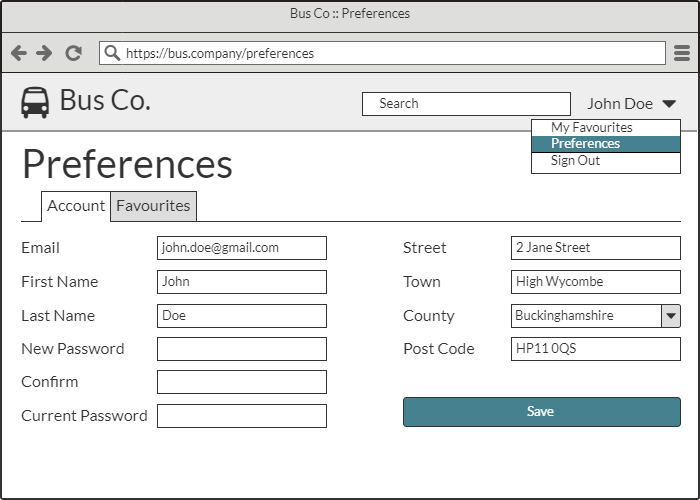
\includegraphics[width=\linewidth]{MockupPreferencesAccount.png}
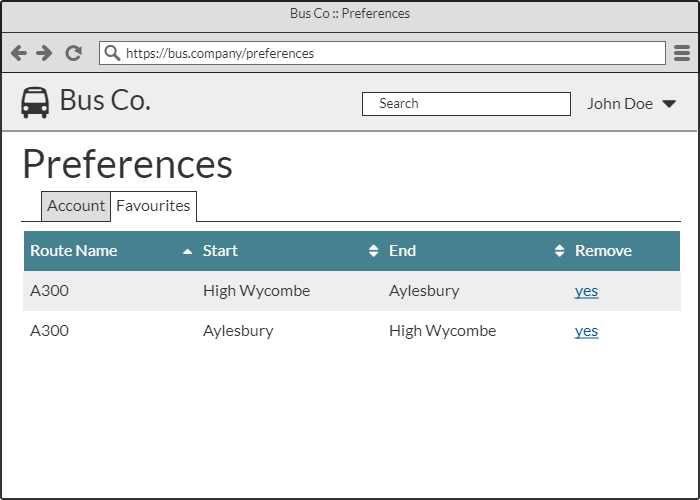
\includegraphics[width=\linewidth]{MockupPreferencesFavourites.png}

\medskip

In the account preferences, users can modify all of their data. If
they set a new password they must enter their current password for
the change to take effect.

\medskip

The favourites tab shows a list of all routes the user has
previously favourited, where they can go to the route details or
remove the route. Removing a route will display a confirmation
prompt to avoid accidental removals.

\subsection{Route Details}

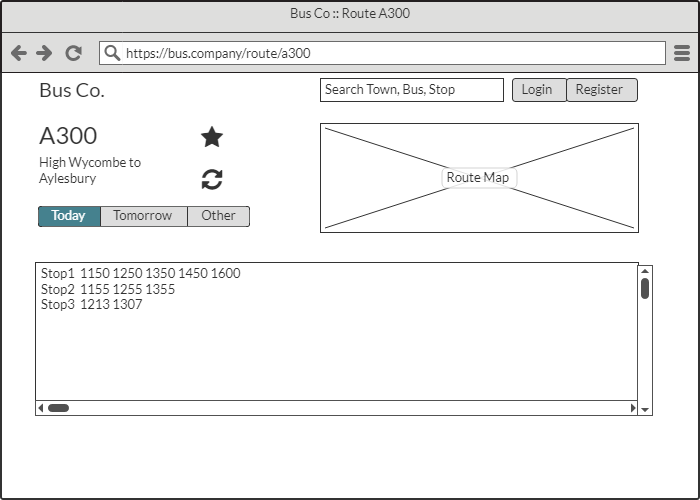
\includegraphics[width=\linewidth]{MockupRouteDetails.png}

\medskip

The route details page shows all the busses running the route with
the estimated time to arrive at each stop along the route.

\medskip

In the top left section, if a user is signed in there will be a
$star$ icon which will add or remove the route from the users
favourites. This icon won't be shown if they are not signed in.

\medskip

Below the route name is the town the route starts and ends in. To
the right of this is an icon to invert the direction, which will
allow the user to see the return times. At the bottom of this
section, there is a series of buttons to switch between showing
route times for the current day, the next day and any other day.
Clicking $Other$ will open a calendar to pick a specific day to
show.

\medskip

On the right is a route map which will show a plotted route with
all the stops using the Google Maps API.

\subsection{Admin Panel}

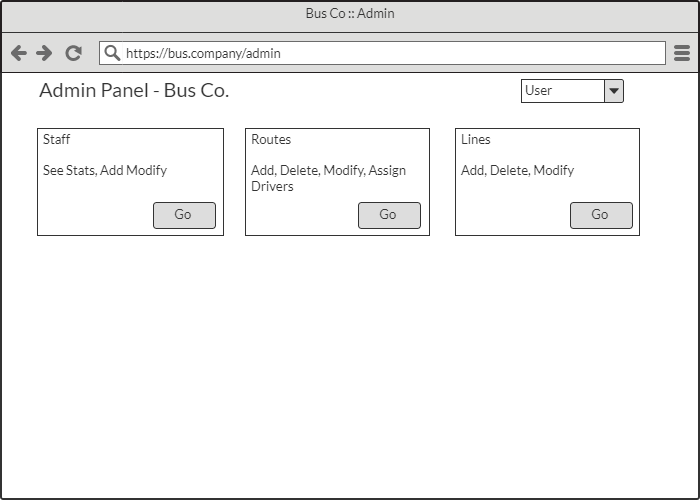
\includegraphics[width=\linewidth]{MockupAdminPanel.png}

\medskip

The admin panel allows staff with the required $Role$(s) to navigate
to the necessary page to edit data in the database directly using
the ASP.NET MVC edit views.

\subsection{Driver Dashboard}

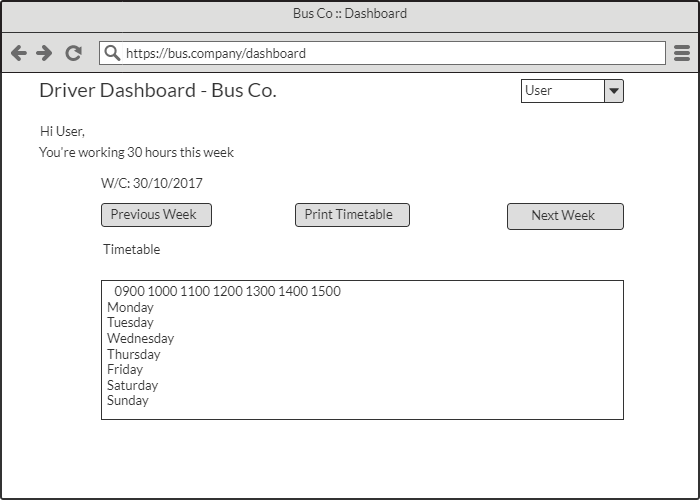
\includegraphics[width=\linewidth]{MockupDriverDashboard.png}

\medskip

The Driver Dashboard is what staff with the $driver$ $Role$ will see
instead of the admin panel. Here they can see the hours they are
assigned for the current week, along with a weekly timetable.

\medskip

The timetable shows the routes they are driving on and at which
times. On desktops, this may show more details such as the bus bay
or town the assigned route is starting and ending in alongside the
route name. Clicking on the route bar will open a modal containing
all the required information and allow the driver to view the
relevant route details page.

\medskip

The driver can also access previous and future weeks, as well as
print a printer-friendly version of the timetable.

\subsection{Line Management}

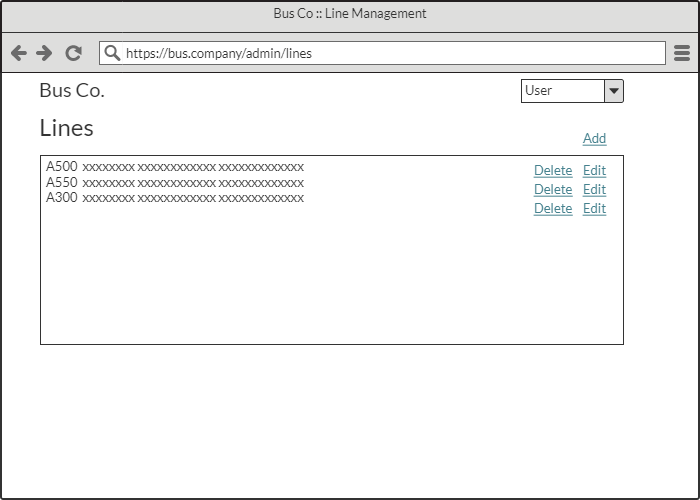
\includegraphics[width=\linewidth]{MockupLineManagement.png}

\medskip

The line management page in the admin panel lists all the lines
operated by the bus company. Key details are shown in this list and
can be deleted or edited by staff members. New lines can be added
by the button in the top right.

\subsection{Route Management}

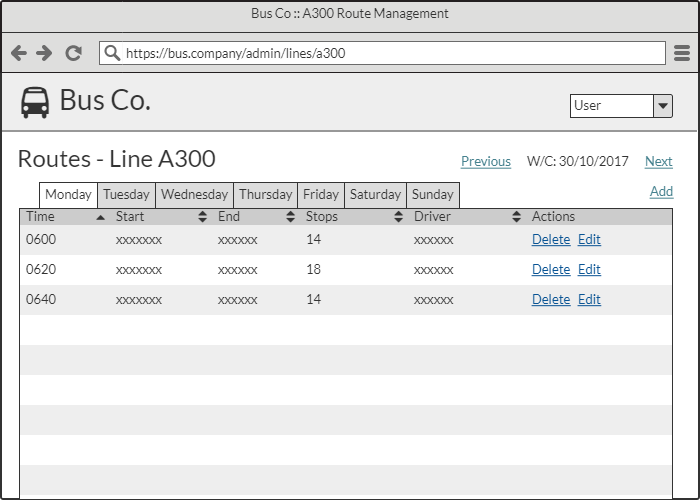
\includegraphics[width=\linewidth]{MockupRouteManagement.png}

\medskip

Route management can be accessed from the $Admin Panel$ or through
the $Line Management$ page.

\medskip

The page shows all the routes assigned to a specific line with their
start times and other important information. It defaults to showing
all the route data for the current week which can be navigated on a
week-by-week basis.

\medskip

New routes can be added to a line here, as well as be removed or
modified.

\subsection{Route Editing}

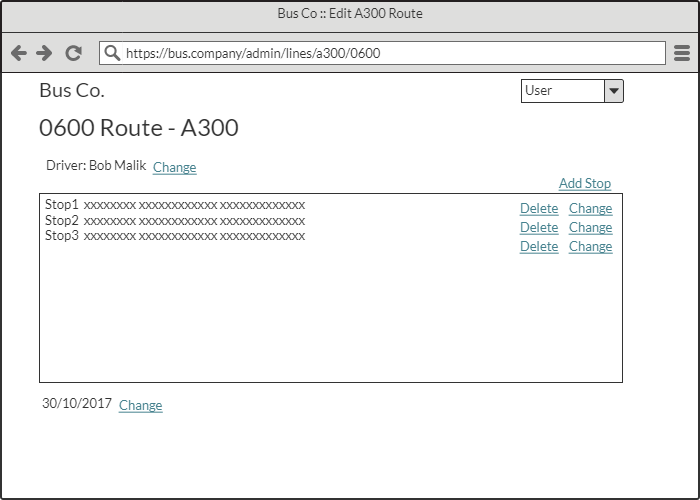
\includegraphics[width=\linewidth]{MockupRouteEditing.png}

\medskip

The route edit page is accessed from clicking the $Edit$ button on a
route in the $Route Management$ page.

\medskip

The driver assigned to the particular route is displayed along with
a list of all the stops assigned to the route. These can be added,
deleted or modified.
